\chapter{\selectlanguage{greek}Θεωρητικό υπόβαθρο}

Στο κεφάλαιο αυτό παρουσιάζονται αναλυτικά οι ...

\section{\selectlanguage{greek}\en{Deep Learning}\cite{LeCun2015}}

Η υπολογιστική εκμάθηση \en{(Machine Learning)} είναι η κινητήριος δύναμη για διάφορες εκφάνσεις της σύγχρονης κοινωνίας: από αναζητήσεις στο διαδίκτυο μέχρι και φιλτράρισμα περιεχομένου σε κοινωνικά δίκτυα και προτάσεις αγορών σε ηλεκτρονικά καταστήματα. 
Ολοένα συχνότερη και συνηθέστερη γίνεται η εμφάνιση του σε προϊόντα ευρείας κατανάλωσης όπως κάμερες και κινητά τηλέφωνα. 
Τα συστήματα υπολογιστικής εκμάθησης χρησιμοποιούνται για την αναγνώριση αντικειμένων σε εικόνες, την αυτόματη καταγραφή προφορικού λόγου, την αντιστοίχηση προϊόντων, νέων, δημοσιεύσεων με τις προτιμήσεις χρηστών. 
Σε όλες αυτές τις εφαρμογές, είναι αυξανόμενη η χρήση ενός σετ τεχνικών που φέρει το όνομα \en{Deep Learning}.

Οι συμβατικές τεχνικές υπολογιστικής εκμάθησης είχαν περιορισμένη δυνατότητα χρήσης της ανεπεξέργαστης πληροφορίας. 
Για δεκαετίες, η σχεδίαση και η υλοποίηση ενός συστήματος αναγνώρισης προτύπων ή υπολογιστικής εκμάθησης, απαιτούσε προσεκτική προσέγγιση και σημαντική εξειδίκευση στον εκάστοτε τομέα. 
Αυτό επειδή χρειαζόταν η μετατροπή της ανεπεξέργαστης πληροφορίας σε μία κατάλληλη εσωτερική αναπαράσταση, την οποία το υποσύστημα εκμάθησης -- συχνότερα ένας ταξινομητής -- θα χρησιμοποιούσε για αναγνωρίσει πρότυπα στις διάφορες εισόδους.

Η εκμάθηση αναπαραστάσεων είναι ένα σύνολο μεθόδων που επιτρέπουν σε ένα σύστημα να ανακαλύψει αυτόματα ποιες ακριβώς αναπαραστάσεις της ανεπεξέργαστης πληροφορίας χρειάζεται για να επιτελέσει την αναγνώριση προτύπων ή την ταξινόμηση. 
Οι μέθοδοι \en{Deep Learning} είναι μέθοδοι εκμάθησης αναπαραστάσεων με πολλαπλά επίπεδα αναπαράστασης, που αποτελούνται από την σύνθεση απλών, μη γραμμικών υποσυστημάτων, το καθένα από τα οποία -- ξεκινώντας από την ανεπεξέργαστη είσοδο -- μετατρέπει την αναπαράσταση της πληροφορίας σε μια λίγο πιο υψηλά αφαιρετική μορφή σε κάθε επίπεδο.
Με την χρήση αρκετών τέτοιων μετατροπών το σύστημα μπορεί να μάθει εξαιρετικά σύνθετες λειτουργίες.
Για διαδικασίες ταξινόμησης, τα υψηλότερα επίπεδα αναπαράστασης ενισχύουν πτυχές τις εισόδου που είναι πιο σημαντικές για τον τελικό σκοπό.
Σε μία εικόνα, για παράδειγμα, η οποία αναπαριστάται ως διάνυσμα τιμών εικονοκυττάρων, τα χαρακτηριστικά που μαθαίνονται στο πρώτο επίπεδο είναι συνήθως πληροφορία για την παρουσία ή την απουσία ακμών σε συγκεκριμένες θέσεις και προσανατολισμούς.
Στο δεύτερο επίπεδο, συνήθως εντοπίζονται μοτίβα μέσω των διαφόρων διατάξεων των ακμών, χωρίς να χρειάζεται τα μοτίβα να επαναλαμβάνονται επακριβώς.
Στο τρίτο επίπεδο μπορούν να αναγνωριστούν σύνολα μοτίβων σε μεγάλους συνδυασμούς που αντιστοιχούν σε γνωστά αντικείμενα ή μέρη τους.
Τα επόμενα επίπεδα, παρόμοια, εντοπίζουν πιο σύνθετα αντικείμενα ως συνδυασμούς απλούστερων μερών.
Το βασικότερο στοιχείο του \en{Deep Learning} είναι πως τα επίπεδα που εντοπίζουν χαρακτηριστικά και δομές δεν είναι σχεδιασμένα από τους ανθρώπους: μαθαίνονται από τα δεδομένα χρησιμοποιώντας γενικευμένες διαδικασίες εκμάθησης.

Η χρήση του \en{Deep Learning} έχει βοηθήσει στην αντιμετώπιση προβλημάτων που δυσκόλευαν την κοινότητα της τεχνητής νοημοσύνης εδώ και χρόνια. 
Αποδεικνύεται να έχει επιδόσεις χωρίς προηγούμενο στον εντοπισμό πολύπλοκων δομών σε δεδομένα πολλών διαστάσεων και για αυτό είναι εφαρμόσιμο σε πολλούς διαφορετικούς τομείς, επιστημονικούς, επιχειρησιακούς και κοινωνικοπολιτικούς.
Πέρα από επαναστατικές επιδόσεις στην αναγνώριση φωνής και εικόνας, έχει ξεπεράσει άλλες τεχνικές υπολογιστικής εκμάθησης στην πρόβλεψη συμπεριφοράς μορίων φαρμάκων, στην ανάλυση δεδομένων από επιταχυντές σωματιδίων, στην ανακατασκευή εγκεφαλικών κυκλωμάτων και στην πρόβλεψη των επιπτώσεων μεταλλάξεων μη κωδικοποιητικού \en{DNA} στις γονιδιακές εκφράσεις και ασθένειες.
Ίσως, οι πιο αναπάντεχα υποσχόμενες επιδόσεις έγιναν στον κλάδο της επεξεργασίας φυσικής γλώσσας, συγκεκριμένα στην εντοπισμό θεμάτων, την ανάλυση συναισθήματος, τις ερωτήσεις - απαντήσεις και την μετάφραση.
%TODO References for best results from paper Deep Learning Hinton Bengio lecun

\section{\selectlanguage{greek}\en{Supervised Learning}\cite{LeCun2015}}

Η πιο συνήθης μορφή υπολογιστικής εκμάθησης, είτε \en{Deep Learning} είτε όχι, είναι αυτή της επιτηρούμενης εκμάθησης.
Ας θεωρήσουμε πως θέλουμε να φτιάξουμε ένα σύστημα που αποφασίζει τι περιέχει μια εικόνα, όπως ένα σπίτι, ένα αυτοκίνητο, έναν άνθρωπο ή μία γάτα.
Αρχικά, συλλέγουμε ένα αρκετά μεγάλο σύνολο δεδομένων με εικόνες στα οποία σημειώνεται τι αντικείμενο από τα παραπάνω περιέχει κάθε εικόνα.
Κατά τη διάρκεια της εκπαίδευσης, δείχνουμε στο σύστημα μια εικόνα και αυτό παράγει μία πρόβλεψη, στη μορφή ενός διανύσματος με σκορ για κάθε κατηγορία.
Θέλουμε η επιθυμητή κατηγορία να έχει το μεγαλύτερο σκορ πρόβλεψης, αλλά αυτό είναι πολύ δύσκολο πριν την εκπαίδευση.
Υπολογίζουμε μία αντικειμενική συνάρτηση με την οποία μετράμε το λάθος (ή την απόσταση) μεταξύ των αποτελεσμάτων του συστήματος και τον επιθυμητών αποτελεσμάτων.
Το σύστημα, ύστερα, προσαρμόζει τις εσωτερικές του παραμέτρους ώστε να μειώσει το λάθος.
Οι εσωτερικές παράμετροι, που συχνότερα στη βιβλιογραφία απαντώνται ως βάρη, είναι πραγματικοί αριθμοί που ορίζουν την λειτουργικότητα εισόδου-εξόδου του συστήματος.
Σε ένα τυπικό \en{Deep Learning} σύστημα, οι εσωτερικές παράμετροι και τα παραδείγματα που χρησιμοποιούμε για την εκμάθηση του συστήματος μπορεί να είναι εκατοντάδες εκατομμύρια σε αριθμό. 

Για την κατάλληλη προσαρμογή των βαρών, ο αλγόριθμος εκμάθησης υπολογίζει ένα διάνυσμα κλίσης, για κάθε βάρος, που δείχνει κατά πόσο και προς ποια κατεύθυνση αλλάζει το λάθος αν αλλάξουμε απειροστά το αντίστοιχο βάρος.
Το διάνυσμα των βαρών τελικά ρυθμίζεται έτσι ώστε να έχει αντίθετη φορά με το διάνυσμα κλίσης.
Η διαδικασία αυτή είναι μία προσπάθεια ελαχιστοποίησης της συνάρτησης λάθους και μεταγενέστερα της μείωσης, κατά μέσο όρο, των λαθών προβλέψεων του συστήματος.

\begin{figure}[tph]
	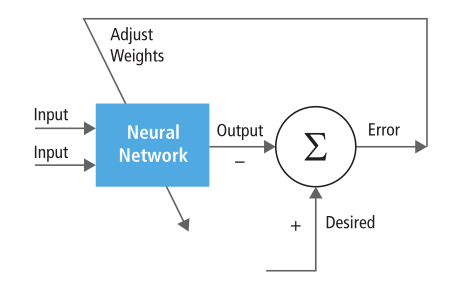
\includegraphics[width=0.8\textwidth, keepaspectratio]{images/training.png}
	\centering 
	\caption{Ένα τυπικό δομικό διάγραμμα επιτηρούμενης εκμάθησης.}
	\label{fig:training}
\end{figure}

Στην πλειοψηφία της σύγχρονης βιβλιογραφίας, και στην παρούσα διπλωματική, ο αλγόριθμος ελαχιστοποίησης που χρησιμοποιείται είναι ο \en{stochastic gradient descent (SGD)}.
Αυτός συνίσταται από την επίδειξη λίγων κάθε φορά, σωστά επισημασμένων, παραδειγμάτων στο σύστημα, τον υπολογισμό των προβλέψεων και του λάθους, τον υπολογισμό του διανύσματος κλίσης και την ρύθμιση των βαρών.
Η παραπάνω διαδικασία επαναλαμβάνεται για πολλά μικρά σετ παραδειγμάτων, μέχρι η συνάρτηση στόχου να σταματήσει να μειώνεται.
Μετά την εκπαίδευση, οι επιδόσεις του συστήματος μετρώνται σε ένα σύνολο διαφορετικών παραδειγμάτων, έτσι ώστε να εξεταστεί η ικανότητα γενίκευσης του συστήματος σε εισόδους που βλέπει για πρώτη φορά.
 %TODO What is an objective function, στοχος
 
\section{\selectlanguage{greek}\en{Recurrent Neural Networks}}

Τα αναδραστικά νευρωνικά δίκτυα (\en{Recurrent Neural Networks - RNNs}) είναι μία προσαρμογή των κλασσικών, πλήρως συνδεδεμένων νευρωνικών δικτύων, έτσι ώστε τα πρώτα να μπορούν να διαχειριστούν ακολουθίες. 
Σε κάθε χρονική στιγμή, τα \en{RNNs} δέχονται μια είσοδο, ενημερώνουν την εσωτερική τους κατάσταση και παράγουν μία έξοδο.
Η πολυδιάστατη εσωτερική κατάσταση, που συχνά απαντάται στη βιβλιογραφία ως κρυφή κατάσταση (\en{hidden state}), και η μη γραμμική εξέλιξη της διαχειριζόμενης πληροφορίας δίνουν στα αναδραστικά νευρωνικά δίκτυα μεγάλη εκφραστική ευελιξία και δυνατότητα ενσωμάτωσης και διατήρησης της πληροφορίας σε μεγάλα χρονικά διαστήματα.
Ακόμα και όταν η μη γραμμική συνάρτηση που χρησιμοποιείται από κάθε στοιχείο του RNN είναι εξαιρετικά απλή, η χρήση της σε πολλά επίπεδα και η επανάληψη της σε κάθε χρονική στιγμή οδηγεί σε ένα εξαιρετικά δυναμικό σύστημα. 

Τα αναδραστικά νευρωνικά δίκτυα ορίζονται ως εξής: δεδομένης μιας ακολουθίας διανυσμάτων εισόδου $(x_1, x_2, ..., x_T)$, το σύστημα υπολογίζει μία ακολουθία κρυφών κατάστασεων $(h_1, h_2, ..., h_T)$ και μία παράγει μια ακολουθία εξόδων $(ο_1, ο_2, ..., ο_T)$, σύμφωνα με τον κάτωθι αλγόριθμο:

\selectlanguage{english}

\begin{algorithmic}
\FOR { $t = 1$ to $T$}
        \STATE \begin{equation}
        	h_t = \tanh(W_h x_t + W_{hh} h_{t-1} + b_h)\label{eq:h}
        	\end{equation}
        	 \STATE \begin{equation}
					o_t = W_{oh} h_t + b_o
        	\end{equation}
\ENDFOR
\end{algorithmic}

\selectlanguage{greek}

Σε αυτές τις εξισώσεις, το $W_{hx}$ είναι ο πίνακας βαρών από την είσοδο στην κρυφή κατάσταση, το $W_{hh}$ είναι ο πίνακας απο την κρυφή κατάσταση στην κρυφή κατάσταση, το $W_{oh}$ είναι ο πίνακας βαρών απο την κρυφή κατάσταση στην έξοδο και τα $b_h, b_o$ είναι οι σταθεροί όροι.
Η μη ορισμένη σχέση $W_{hh}h_{t-1}$ στη χρονική στιγμή $t = 1$ αντικαθιστάται με ένα διάνυσμα αρχικοποίησης, $h_{init}$, και η συνάρτηση της υπερβολικής εφαπτομένης, $\tanh$, εφαρμόζεται κατά στοιχείο.

\begin{figure}[tph]
	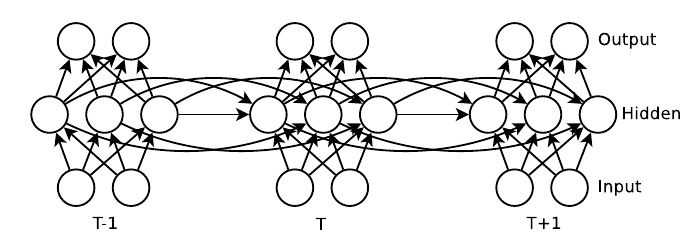
\includegraphics[width=\textwidth, keepaspectratio]{images/rnn.png}
	\centering 
	\caption{Ένα αναδραστικό νευρωνικό δίκτυο είναι ένα πολύ <<βαθύ>> πλήρως συνδεδεμένο νευρωνικό 			δίκτυο του οποία τα βάρη επαναχρησιμοποιούνται στις διάφορες χρονικές στιγμές. Η μη 					γραμμική συνάρτηση ενεργοποίησης που χρησιμοποιεί η κρυφή κατάσταση είναι η πηγή της 					πλούσιας δυναμικής του συστήματος.}
	\label{fig:rnn}
\end{figure}

Οι παράγωγοι των στοιχειδών μερών του δικτύου είναι εύκολο να υπολογιστούν, με τη μέθοδο της προς τα πίσω διάδοσης σφάλματος, \cite{Graves2013}, \cite{Rieman2014} οπότε ίσως η εκπαίδευση ενός τέτοιου συστήματος φαίνεται εύκολη.
Στην πραγματικότητα, η σχέση μεταξύ των παραμέτρων του RNN και της δυναμικής του είναι εξαιρετικά ασταθής, γεγονός που καθιστά τον αλγόριθμο \en{SGD} αναποτελεσματικό.
Αυτό τεκμηριώνεται απο \cite{tofill} και \cite{tofill} που αποδεικνύουν οτι τα διανύσματα κλίσεων τείνουν να μηδενίζονται (ή σπανιότερα να απειρίζονται) εκθετικά με την διάδοση του σφάλματος στο χρόνο.
Στη σχετική βιβλιογραφία αυτό απαντάται ως πρόβλημα εξαφάνισης ή έκρηξης των διανυσμάτων κλίσης (<<\en{vanishing or exploding gradients problem}>>)
Το παραπάνω χρησιμοποιήθηκε ως επιχείρημα για το οτι τα αναδραστικά νευρωνικά δίκτυα δεν μπορούν να αποτυπώσουν εξαρτήσεις με μεγάλη χρονική απόσταση μεταξύ τους, οταν ο χρησιμοποιείται ο αλγόριθμος \en{SGD}.
Επιπρόσθετα, ο περιστασιακός απειρισμός των διανυσμάτων κλίσης αυξάνει τη διακύμανση τους και κάνει την εκμάθηση ασταθή.
Τα θεωρητικά αποτελέσματα αυτά, δεδομένου πως ο \en{SGD} ήταν ο βασικότερος αλγόριθμος εκπαίδευσης νευρωνικών δικτύων, σε συνδυασμό με την εμπειρική δυσκολία εκπαίδευσης των \en{RNNs} οδήγησε στη σχεδόν ολοκληρωτική εγκατάλειψη της σχετικής έρευνας.

\section{\selectlanguage{greek}Εκπαίδευση των \en{Recurrent Neural Networks}}
\subsection{\en{Long Short-Term Memory Units}\cite{Hochreiter1997}}

Ένας τρόπος να αντιμετωπιστεί η αδυναμία που παρουσιάζουν τα RNNs στη δυσκολία εκμάθησης δομών με μακρινές, στο χρόνο, αλληλεξαρτήσεις είναι η τροποποίηση του μοντέλου ώστε να έχει στοιχεία με μνήμη.
Η προσέγγιση αυτή ονομάζεται \en{Long Short-Term Memory} και γνωρίζει ευρεία χρήση. Οι σχέσεις που ορίζουν κάθε στοιχείο μνήμης είναι:

\begin{equation}
i_t = \sigma{(W_{xi}x_t + W_{hi}h_{t-1} + W_{ci}c_{t-1} + b_i)}
\end{equation}
\begin{equation}
f_t = \sigma{(W_{xf}x_t + W_{hf}h_{t-1} + W_{cf}c_{t-1} + b_f)}
\end{equation}
\begin{equation}
c_t = f_t c_{t-1} + i_t \tanh{(W_{xc} h_{t-1} + W_{cf} c_{t-1} + b_c)}\label{eq:c}
\end{equation}
\begin{equation}
o_t = \sigma(W_{xo}x_t + W_{ho} h_{t-1} + W_{co} c_t + b_o)
\end{equation}
\begin{equation}
h_t = o_t\tanh{c_t}
\end{equation}

όπου το $\sigma$ είναι η σιγμοειδής συνάρτηση, $i, f, o$ και $c$ είναι αντίστοιχα η πύλη εισόδου, η πύλη απώλειας μνήμης, η πύλη εξόδου και η μνήμη.
Τα τελευταία είναι διανύσματα με διαστάσεις ίδιες με του διανύσματος $h$ (βλ. εξίσωση \ref{eq:h}, που ταυτίζεται με τον δέυτερο όρο της εξίσωσης \ref{eq:c}). 
...

Μια πιο διαισθητική εξήγηση του συστήματος \en{LSTM} είναι
